\newpage
\section{反步法(Backstepping)}\label{5Dref}
\subsection{基本反步法}
考虑系统
\begin{equation}
    \begin{aligned}
  \dot{z} & = f (z) + g (z) \xi\\
  \dot{\xi} & = u
\end{aligned}\label{Sys:backstep:basic:original}
\end{equation}
其中 $[z^T, \xi^T]^T \in \mathbf{R}^{n + 1}$ 为状态,$u \in
\mathbf{R}$ 为控制输入。函数$f, g$在包含$z = 0$的域$D$上光滑,且有 $f (0) = 0$。

我们的目标是设计状态反馈控制律以镇定原点。%将原系统看作两个系统之级联。

假设我们能通过一反馈控制律$\xi = \Phi (z)$($\Phi (0) = 0$)来渐近镇定{\bf 第一个系统}(将$\xi$看作虚拟的控制输入),也就是使
\begin{equation}
    \dot{z} = f (z) + g (z) \Phi (z) \label{first_stablize}
\end{equation}
的原点是渐近稳定的。于是,我们可知一定存在 Lyapunov 函数 $V (z)$ 使得
\[ \dot{V} = \frac{\partial V}{\partial z} [f (z) + g (z) \Phi (z)] \leq -
   \omega (z) \]
其中 $\omega (z)$ 正定。

在原系统中加减$g (z) \Phi (z)$,凑出 \eqref{first_stablize} 的形式
\begin{equation}
   \begin{aligned}
  \dot{z} & = f (z) + g (z) \Phi (z) + g (z) (\xi - \Phi (z))\\
  \dot{\xi} & = u
\end{aligned} \label{Sys:backstep:basic:control}
\end{equation}

引入状态变换(表征“真实的”$\xi$和“理想的”$\xi=\Phi (z)$之间的差异)
\[ y = \xi - \Phi (z) \]
这样,我们如果让$y\to 0$,那么$\xi$就能跟踪理想的控制律$\Phi$,$z$也按上面原点渐近稳定的系统之规律变化。
于是,原系统变为
\begin{equation}
    \begin{aligned}
  \dot{z} & = f (z) + g (z) \Phi (z) + g (z) y\\
  \dot{y} & = \dot{\xi}-\dot{\Phi} (z) = u - \dot{\Phi} (z)
\end{aligned}\label{Sys:backstep:basic:backstep}
\end{equation}
此种状态变换常称作 {\textbf{反步法(backstepping)}}\index{反步法(backstepping)},因为它将控制$- \Phi (z)$“反挪”(back-steps)到了积分之前。

\begin{figure}[htbp]
    \centering
    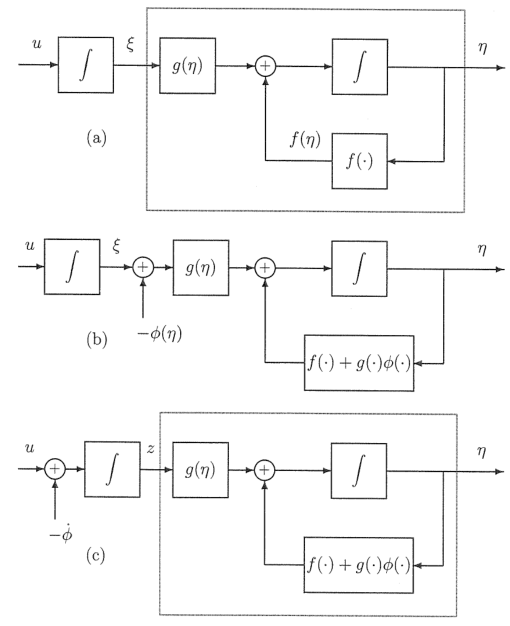
\includegraphics[width=0.5\linewidth]{figure/adaptive/backstepping.png}
    \caption{反步法示意图。图中的$\eta$为此处的$z$。(a) 原系统 \eqref{Sys:backstep:basic:original};(b) 引入控制$\Phi(z)$,即 \eqref{Sys:backstep:basic:control};(c) 将$\Phi(z)$“反挪”(back-steps)到积分之前,即 \eqref{Sys:backstep:basic:backstep}。}
    \label{fig:backstepping}
\end{figure}

因为 $f, g$ 与 $\Phi$ 已知,所以可求出
\[ \dot{\Phi} (z) = \frac{\partial \Phi}{\partial z} \dot{z} = \frac{\partial
   \Phi}{\partial z} (f (z) + g (z) \xi) \]
令 $v = u - \dot{\Phi} (z)$(“新的”控制输入),将上述系统简化成
\begin{align*}
  \dot{z} & = f (z) + g (z) \Phi (z) + g (z) y\\
  \dot{y} & = v
\end{align*}
% 这与我们一开始讨论的系统形式大体相同,当$y=0$时第一式中多余的项消失,$z$的原点便渐近稳定。which has the same ``form'' as the system we started with the exception that
% we know the first component is asymptotically stable at the origin when $y$ is zero.

考虑如下候选的合并Lyapunov 函数(combined Lyapunov function candidate,意即将新状态合并进来)
\[ V_c (z, y) = V (z) + \frac{1}{2} y^2 \]
求其导数得
\begin{align*}
  \dot{V}_c (z, y) & = V (z) + y \cdot \dot{y}\\
  & = \frac{\partial V}{\partial z} [f (z) + g (z) \Phi (z) + g (z) y] + y 
  v\\
  & \leq - \omega (z) + \frac{\partial V}{\partial z} g (z) y + y  v
\end{align*}
则取 \[v = - \frac{\partial V}{\partial z} g (z) - k  y, k > 0\]
即可得到\[\dot{V} (z, y) \leq - \omega (z) - k  y^2\]
它是负定的,
这也就表明上述系统的原点 $(z = 0, y = 0)$ 是渐近稳定的。因为
$\Phi (0) = 0$,所以$z = 0, y = 0\implies \xi =0$,即原系统的原点$(z = 0, \xi = 0)$ 是渐近稳定的。整理得到反馈控制律为
\begin{align*}
  u & = v + \dot{\Phi}(z)\\
  & = - \frac{\partial V}{\partial z} g (z) - k  y + \frac{\partial
  \Phi}{\partial z} (f (z) + g (z) \xi)\\
  & = - \frac{\partial V}{\partial z} g (z) - k  (\xi - \Phi (z)) +
  \frac{\partial \Phi}{\partial z} (f (z) + g (z) \xi)
\end{align*}
\begin{example}[利用反步法进行非线性系统设计]
  考虑下述系统
  \begin{align*}
    \dot{x}_1 & = x^2_1 - x^3_1 + x_2\\
    \dot{x}_2 & = u
  \end{align*}
 首先考虑第一个方程,这时将 $x_2$ 视为虚拟的控制输入,先设计反馈控制律 $\Phi (x_1)$(虚拟的$x_2$) 来镇定 $x_1 = 0$。
  
  设计 $\Phi (x_1) = - x^2_1$,我们有 $\dot{x}_1 = - x^3_1$(将稳定的$- x^3_1$保留)。考虑Lyapunov函数
  $V (x_1) = \frac{1}{2} x^2_1$,求其导数得
  \[ \dot{V} (x_1) = x_1 \dot{x}_1 = - x^4_1 \]
  其为负定。
  
  下面应用反步法。选取状态变换(“真实的”$x_2$和“理想的”$x_2$之间的差异)
  \[ y = x_2 - \Phi (x_1) = x_2 + x^2_1 \]
  那么原系统可写为下述形式
  \begin{align*}
    \dot{x}_1 & = - x^3_1 + y\\
    \dot{y}  & = v
  \end{align*}
  其中 $v = u + 2 x_1 (x^2_1 - x^3_1 + x_2)$。
  
  接下来,我们考虑如下候选合并Lyapunov 函数
  \[ V_c = \frac{1}{2} x^2_1 + \frac{1}{2} y^2 \]
  其导数为
  \begin{align*}
    \dot{V}_c & = x_1 \dot{x}_1 + y  \dot{y} = - x^4_1 + x_1 y + y  v
  \end{align*}
  选取 $v = - x_1 - k  y, k > 0$,那么 $\dot{V}_c = - x^4_1 - k  y^2$ 负定。
  因此, $x_1, y \rightarrow 0$,也就说明$x_1,x_2\rightarrow 0$。
  
  整理得控制输入如下
  \[ u = v - 2 x_1 (x^2_1 - x^3_1 + x_2) = - x_1 - k  y - 2 x_1 (x^2_1 - x^3_1
     + x_2) \]
\end{example}

\begin{problem}
如果系统不是由二个系统级联
    \begin{align*}
    \dot{x}_1 & = x^2_1 - x^3_1 + x_2\\
    x_2 & = - x^2_1 + x_1 x_2 + \cdots \\
    \dot{x}_3 & = u
  \end{align*}
  甚或并不存在$\dot{x}_i=u$的项
  \begin{align*}
    \dot{x}_1 & = -x_1^2+ x_2+\sin x_1\\
    x_2 & = \cos x_2^2 + x_3+ \cdots \\
    \dot{x}_3 & = u +\sin x_2 -x_1^2+ \cdots 
  \end{align*}
  如何进行设计?
\end{problem}

\subsection{自适应反步法}

考虑如下系统
\begin{equation}
    \begin{aligned}
  \dot{x}_1 & = x_2 + \varphi (x_1) \theta\\
  \dot{x}_2 & = u
\end{aligned}\label{Sys:adaptive_backstepping}
\end{equation}
其中 $\theta$ 为未知常数,$\varphi (x_1)$ 是有界函数,$\varphi (0) = 0$。

不妨假设 $\theta$ 已知。若将$x_2$看作控制输入,理想情况下其应设计为
\[- k_1 x_1 - \varphi (x_1) \theta \triangleq \alpha_1 (x_1,\theta), k_1 > 0
\]
但是, $\theta$ 未知。不过,引入自适应控制思想,仍可应用反步法。

\noindent{\textbf{步骤 1: }}

定义 $z_1 = x_1$,将$x_2$看作控制输入。因为$\theta$ 未知,设计自适应律($v_1$即 $\theta$的状态估计$\hat{\theta}$)
\begin{align*}
  \alpha_1 (x_1, v_1) & = - k_1 z_1 - \varphi (z_1) v_1
\end{align*}
并定义状态变换(“真实的”$x_2$减去“理想的”$x_2$)
\[ z_2 \triangleq x_2 - \alpha_1 (x_1, v_1) \]
于是$z_1$的动力学写为
\begin{align*}
  \dot{z}_1 & = \dot{x}_1\\
  & = x_2 + \varphi (z_1) \theta\\
  & = x_2 - \alpha_1 (x_1, v_1) + \alpha_1 (x_1, v_1) + \varphi (z_1)
  \theta\\
  & = z_2 - k_1 z_1 - \varphi (z_1) (v_1 - \theta)
\end{align*}
考虑如下候选 Lyapunov 函数(欲使$x_1$与参数估计误差趋于$0$)
\[ V_1 (z_1, v_1) = \frac{1}{2} z^2_1 + \frac{1}{2 \gamma_1} (v_1 - \theta)^2
\]
求其导数得到
\begin{align*}
  \dot{V}_1 & = z_1 \dot{z}_1 + \frac{1}{\gamma_1} (v_1 - \theta)
  \dot{v}_1\\
  & = z_1 (z_2 - k_1 z_1 - \varphi (z_1) (v_1 - \theta)) +
  \frac{1}{\gamma_1} (v_1 - \theta) \dot{v}_1\\
  & = -k_1z_1^2+z_1z_2+\frac{1}{\gamma_1} (v_1-\theta)(-\gamma_1z_1\varphi (z_1) +\dot{v}_1)
\end{align*}
设计
\[\dot{v}_1 = \gamma_1 z_1 \varphi (z_1)\]
则
\begin{align*}
  \dot{V}_1 &  = - k_1 z^2_1 + z_1 z_2
\end{align*}

\noindent{\textbf{步骤 2: }}

$z_2$的动力学写为
  \begin{align*}
  \dot{z}_2 & = \dot{x}_2 - \dot{\alpha}_1 (z_1, v_1)\\
  & = u - \frac{\partial \alpha_1}{\partial z_1} \dot{z}_1 - \frac{\partial
  \alpha_1}{\partial v_1} \dot{v}_1\\
  & = u - \frac{\partial \alpha_1}{\partial z_1} (x_2 + \varphi (z_1)
  \theta) - \frac{\partial \alpha_1}{\partial v_1} \gamma_1 z_1 \varphi
  (z_1)\\
  & = u - \frac{\partial \alpha_1}{\partial z_1} x_2 - \frac{\partial
  \alpha_1}{\partial v_1} \gamma_1 z_1 \varphi (z_1) - \theta \frac{\partial
  \alpha_1}{\partial z_1} \varphi (z_1)
\end{align*}
接下来,我们尝试选取一候选Lyapunov函数并设计$u$,使得闭环系统是渐近稳定的。
首先尝试考察下列候选合并Lyapunov函数(为何是“尝试”?请注意上式中含有的未知参数$\theta$)
\[ V_c (z_1, z_2, v_1) = V_1 (z_1, v_1) + \frac{1}{2} z^2_2 \]
求其导数得
\begin{align*}
  \dot{V}_c & = \dot{V}_1 + z_2 \dot{z}_2\\
  & = - k_1 z^2_1 + \textcolor{red}{z_1 z_2} + z_2 \left( u \textcolor{structurecolor}{- \frac{\partial
  \alpha_1}{\partial z_1} x_2 - \frac{\partial \alpha_1}{\partial v_1}
  \gamma_1 z_1 \varphi (z_1)} \textcolor{second}{- \theta \frac{\partial \alpha_1}{\partial z_1}  \varphi (z_1)} \right)
\end{align*}
为了处理含有未知参数$\theta$的项,我们尝试利用先前对$\theta$作出的估计$v_1$,写出(请注意,与上式的颜色对应之项会被消去)
\[ u = \textcolor{red}{- z_1} - k_2 \textcolor{structurecolor}{+ \frac{\partial \alpha_1}{\partial z_1} x_2 +
   \frac{\partial \alpha_1}{\partial v_1} \gamma_1 z_1 \varphi (z_1)} \textcolor{second}{+ v_1
   \frac{\partial \alpha_1}{\partial z_1} \varphi (z_1)}, k_2 > 0 \]
于是可得
\[ \dot{V}_c = - k_1 z^2_1 - k_2 z^2_2 + z_2 (v_1 - \theta) \frac{\partial
   \alpha_1}{\partial z_1} \varphi (z_1) \]
然而,我们已无消去含 $(v_1 - \theta)$项的余地了。为了解决该问题,对$\theta$引入一新的估计$v_2$,写出
\[ u = - z_1 - k_2 + \frac{\partial \alpha_1}{\partial z_1} x_2 +
   \frac{\partial \alpha_1}{\partial v_1} \gamma_1 z_1 \varphi (z_1) + v_2
   \frac{\partial \alpha_1}{\partial z_1} \varphi (z_1), k_2 > 0 \]
新出现的 $v_2$,表明候选Lyapunov函数应改为(最后一项是$v_2$对$\theta$的参数估计误差)
\begin{align*}
  V_c & = V_1 (z_1, v_1) + \frac{1}{2} z^2_2 + \frac{1}{2 \gamma_2} (v_2 -
  \theta)^2
\end{align*}
根据上述控制律,其导数为
\[ \dot{V}_c = - k_1 z^2_1 - k_2 z^2_2 + z_2 (v_2 - \theta) \frac{\partial
   \alpha_1}{\partial z_1} \varphi (z_1) + \frac{1}{\gamma_2} (v_2 - \theta)
   \dot{v}_2 \]
这样,选取\[\dot{v}_2 = - \gamma_2 z_2 \frac{\partial \alpha_1}{\partial z_1}
\varphi (z_1)\]以使后两项相消,即可得到$\dot{V}_c = - k_1 z^2_1 - k_2 z^2_2$,其为负半定。对该导数式两边积分可得
\[ k_1 \int^t_0 z^2_1 \diff \tau + k_2 \int^t_0 z^2_2 \diff \tau = V_c (0) - V_c (t)  \leq V_c (0) \]
则得 $z_1, z_2 \in \mathbf{L}_2 \cap \mathbf{L}_{\infty}$。又$\dot{z}_1,
\dot{z}_2 \in \mathbf{L}_{\infty}$,
根据 \ref{barbalat_cor_1},$\lim\limits_{t \rightarrow \infty} z_1 = \lim\limits_{t \rightarrow
\infty} z_2 = 0$。
又注意到 $z_1 = x_1, x_2 = z_2 - \alpha_1 (x_1, v_1)$ 且 $\varphi (0) = 0$,于是可得出结论 $\lim\limits_{t \rightarrow \infty} x_1 = \lim\limits_{t \rightarrow \infty} x_2 = 0$。
\begin{note}
    施加自适应律的闭环系统方程是
\begin{align*}
  \dot{z}_1 & = - k_1 z_1 + z_2 - (v_1 - \theta) \varphi (z_1)\\
  \dot{z}_2 & = - z_1 - k_2 z_2 + (v_2 - \theta) \frac{\partial
  \alpha_1}{\partial z_1} \varphi (z_1)\\
  \dot{v}_1 & = \gamma_1 z_1 \varphi (z_1)\\
  \dot{v}_2 & = - \gamma_2 z_2 \frac{\partial \alpha_1}{\partial z_1}
  \varphi (z_1)
\end{align*}
写成矩阵形式是
\begin{align*}
  \left[\begin{array}{c}
    \dot{z}_1\\
    \dot{z}_2
  \end{array}\right] & = \left[\begin{array}{cc}
    - k_1 & 1\\
    - 1 & - k_2
  \end{array}\right] \left[\begin{array}{c}
    z_1\\
    z_2
  \end{array}\right] + \left[\begin{array}{cc}
    - \varphi (z_1) & 0\\
    0 & \frac{\partial \alpha_1}{\partial z_1} \varphi (z_1)
  \end{array}\right] \left[\begin{array}{c}
    v_1 - \theta\\
    v_2 - \theta
  \end{array}\right]\\
  \left[\begin{array}{c}
    \dot{v}_1\\
    \dot{v}_2
  \end{array}\right] & = - \left[\begin{array}{cc}
    \gamma_1 & 0\\
    0 & \gamma_2
  \end{array}\right] \left[\begin{array}{cc}
    - \varphi (z_1) & 0\\
    0 & \frac{\partial \alpha_1}{\partial z_1} \varphi (z_1)
  \end{array}\right] \left[\begin{array}{c}
    z_1\\
    z_2
  \end{array}\right]
\end{align*}
\end{note}

\begin{problem}
  \[ \left\{\begin{array}{l}
       \dot{x}_1 = x_2 + \theta_1 \varphi_1 (x_1)\\
       \dot{x}_2 = u + \theta_2 \varphi_2 (x_2)
     \end{array}\right. \]
  设计 $u$以镇定该系统。
\end{problem}
\begin{hint}
    消去已知的多余项,对于未知参数使用自适应方法估计。
\end{hint}

\subsection{减少过参数化(Reduce the overparametrization)}

上述方法对于同一个未知参数要进行两次估计。下面介绍的方法仅需估计一次。仍考虑系统 \eqref{Sys:adaptive_backstepping}。接下来,为求简便,$\varphi(z_1)=\varphi(x_1)$简写为$\varphi$。

\noindent{\textbf{步骤 1: }}

定义 $z_1 = x_1$,并将$x_2$视为控制输入,应用自适应控制思想对未知参数进行估计
\begin{equation*}
   - k_1 x_1 - \varphi \hat{\theta} \triangleq \alpha_1 (x_1,
  \hat{\theta}),k_1>0
\end{equation*}
仍定义 $z_2 = x_2 - \alpha_1 (x_1, \hat{\theta})$,有
\begin{align*}
  \dot{z}_1 & = x_2 + \varphi \theta\\
  & = x_2 - \alpha_1 (x_1, \hat{\theta}) + \alpha_1 (x_1, \hat{\theta}) +
  \varphi \theta\\
  & = z_2 - k_1 z_1 - \varphi \tilde{\theta}
\end{align*}
其中 $\tilde{\theta} \triangleq \hat{\theta} - \theta$。与之前方法不同的是,我们并不在这一步就将 $\dot{\hat{\theta}}$设计出来。

\noindent{\textbf{步骤 2: }}

$z_2$的动力学现表示为
\begin{align*}
  \dot{z}_2 & = \dot{x}_2 - \dot{\alpha}_1 (x_1, \hat{\theta})\\
  & = u - \frac{\partial \alpha_1}{\partial z_1} \dot{z}_1 - \frac{\partial
  \alpha_1}{\partial \hat{\theta} } \dot{\hat{\theta}} \\
  & = u - \frac{\partial \alpha_1}{\partial z_1} (z_2 - k_1 z_1 - \varphi
  \tilde{\theta}) + \varphi \dot{\hat{\theta} }
\end{align*}
考虑下述候选合并Lyapunov函数
\[ V_c = \frac{1}{2} z^2_1 + \frac{1}{2} z^2_2 + \frac{1}{2 \gamma }
   \tilde{\theta}^2 \]
其导数为
\begin{align*}
  \dot{V}_c & = z_1 \dot{z}_1 + z_2 \dot{z}_2 + \frac{1}{\gamma}
  \tilde{\theta} \dot{\hat{\theta}}\\
  & = z_1 (z_2 - k_1 z_1 - \varphi \tilde{\theta}) + z_2 \left( u -
  \frac{\partial \alpha_1}{\partial z_1} (z_2 - k_1 z_1 - \varphi
  \tilde{\theta}) + \varphi \dot{\hat{\theta} } \right) + \frac{1}{\gamma}
  \tilde{\theta} \dot{\hat{\theta}}\\
  & = - k_1 z^2_1 + \frac{\tilde{\theta}}{\gamma} \left( \dot{\hat{\theta}}
  - \gamma \varphi z_1 + \gamma z_2 \varphi \frac{\partial \alpha_1}{\partial
  z_1} \right) + z_2 \left( u - \frac{\partial \alpha_1}{\partial z_1} z_2 +
  \frac{\partial \alpha_1}{\partial z_1} k_1 z_1 + z_1 + \varphi
  \dot{\hat{\theta} } \right)
\end{align*}
于是我们选取
\[ \dot{\hat{\theta}} = \gamma \varphi z_1 - \gamma z_2 \varphi \frac{\partial
   \alpha_1}{\partial z_1} \]
\[ u = \frac{\partial \alpha_1}{\partial z_1} z_2 - \frac{\partial
   \alpha_1}{\partial z_1} k_1 z_1 - z_1 - \varphi \dot{\hat{\theta} } - k_2
   z_2, k_2 > 0 \]
即得
\[ \dot{V}_c = - k_1 z^2_1 - k_2 z^2_2 \]
同上一节的分析可知$\lim\limits_{t \rightarrow \infty} z_1 = \lim\limits_{t \rightarrow
\infty} z_2 =\lim\limits_{t \rightarrow \infty} x_1 = \lim\limits_{t \rightarrow \infty} x_2 = 0$。
\begin{note}
    施加自适应律的闭环系统方程是
\begin{align*}
  \dot{z}_1 & = - k_1 z_1 + z_2 - \tilde{\theta} \varphi\\
  \dot{z}_2 & = - z_1 - k_2 z_2 + \tilde{\theta} \frac{\partial
  \alpha_1}{\partial z_1} \varphi\\
  \dot{\hat{\theta}} & = \gamma \varphi z_1 - \gamma z_2 \varphi
  \frac{\partial \alpha_1}{\partial z_1}
\end{align*}
矩阵形式为
\begin{align*}
  \left[\begin{array}{c}
    \dot{z}_1\\
    \dot{z}_2
  \end{array}\right] & = \left[\begin{array}{cc}
    - k_1 & 1\\
    - 1 & - k_2
  \end{array}\right] \left[\begin{array}{c}
    z_1\\
    z_2
  \end{array}\right] + \left[\begin{array}{c}
    - \varphi\\
    \frac{\partial \alpha_1}{\partial z_1} \varphi
  \end{array}\right] \tilde{\theta}\\
  \dot{\hat{\theta}} & = - \gamma \left[\begin{array}{cc}
    - \varphi & \frac{\partial \alpha_1}{\partial z_1} \varphi
  \end{array}\right] \left[\begin{array}{c}
    z_1\\
    z_2
  \end{array}\right]
\end{align*}
\end{note}
\subsection{有调节函数(tuning function)的自适应反步法}
考虑下述系统
\begin{equation}
    \begin{aligned}
        \dot{x}_1&=x_2+\varphi(x_1)\theta\\
        \dot{x}_2&=x_3\\
        \dot{x}_3&=u
    \end{aligned}\label{Sys:tuning}
\end{equation}
其中$\theta$为未知常数,$\varphi(x_1)$为有界函数,$\varphi(0)=0$。

\noindent{\textbf{步骤 1: }}

定义 $z_1 = x_1$,并将$x_2$视为控制输入,理想的$x_2$为
\begin{equation*}
 \alpha_1 (x_1,\hat{\theta}) \triangleq  - k_1 x_1 - \varphi (x_1) \hat{\theta} ,k_1>0
\end{equation*}
仍定义 $z_2 = x_2 - \alpha_1 (x_1, \hat{\theta})$,同上一节有
\begin{align*}
  \dot{z}_1 & = z_2 - k_1 z_1 - \varphi \tilde{\theta}
\end{align*}
其中 $\tilde{\theta} \triangleq \hat{\theta} - \theta$。

考虑候选Lyapunov函数
\[ V_1=\frac12z_1^2+\frac{1}{2\gamma}\tilde{\theta}^2\]
其导数为\begin{align*}
    \dot{V}_1&=z_1\dot{z}_1+\frac{1}{\gamma}\tilde{\theta}\dot{\hat{\theta}}\\
    &=-k_1z_1^2-\varphi(z_1)z_1\tilde{\theta}+z_1z_2+\frac{1}{\gamma}\tilde{\theta}\dot{\hat{\theta}}\\
    &=-k_1z_1^2+z_1z_2+\frac{1}{\gamma}\tilde{\theta}(\dot{\hat{\theta}}-\gamma \varphi(z_1)z_1)
\end{align*}

定义$\tau_1(z_1)=z_1\varphi(z_1)$,称其为{\bf 调节函数(tuning function)}\index{条@调节函数(tuning function)}。

\noindent{\textbf{步骤 2: }}

现对 \eqref{Sys:tuning} 的第二个方程进行设计。将$x_3$看作虚拟控制输入。定义$z_3 = x_3 - \alpha_2 (x_1,x_2, \hat{\theta})$。$z_2$的动力学表示为
\begin{align*}
  \dot{z}_2 & = \dot{x}_2 - \dot{\alpha}_1 (x_1, \hat{\theta})\\
  & = x_3 - \frac{\partial \alpha_1}{\partial z_1} (x_2+\varphi(z_1)\theta)- \frac{\partial
  \alpha_1}{\partial \hat{\theta} } \dot{\hat{\theta}} \\
  & = z_3+\alpha_2(x_1,x_2, \hat{\theta}) - \frac{\partial \alpha_1}{\partial z_1} x_2 - \frac{\partial \alpha_1}{\partial z_1}\varphi(z_1)
  \theta - \frac{\partial
  \alpha_1}{\partial \hat{\theta} } \dot{\hat{\theta}}
\end{align*}
考虑下述候选合并Lyapunov函数
\[ V_2 = V_1 + \frac{1}{2} z^2_2 \]
其导数为
\begin{align*}
    \dot{V}_2&=\dot{V}_1+z_2\dot{z}_2\\
    &=-k_1z_1^2+z_1z_2+\frac{1}{\gamma}\tilde{\theta}(\dot{\hat{\theta}}-\gamma \tau_1(z_1))\\
    &\quad +z_2\left(z_3+\alpha_2(x_1,x_2, \hat{\theta}) - \frac{\partial \alpha_1}{\partial z_1} x_2 - \frac{\partial \alpha_1}{\partial z_1}\varphi(z_1) \theta - \frac{\partial
  \alpha_1}{\partial \hat{\theta} } \dot{\hat{\theta}}\right)
\end{align*}
设计\[\alpha_2=-k_2z_2-z_1+\frac{\partial \alpha_1}{\partial z_1} x_2 +\frac{\partial \alpha_1}{\partial z_1}\varphi(z_1) \textcolor{red}{\hat\theta}+\frac{\partial
  \alpha_1}{\partial \hat{\theta} } \gamma \textcolor{red}{\tau_2}\]
注意其中的$\theta$以其估计代之;最后一项新增一个调节函数$\tau_2$。这样上面的$\dot{V}_2$就写为
\begin{align*}
    \dot{V}_2&=-k_1z_1^2-k_2z_2^2+z_2z_3+\frac{1}{\gamma}\tilde{\theta}(\dot{\hat{\theta}}-\gamma \tau_1(z_1))+z_2\frac{\partial \alpha_1}{\partial z_1}\varphi(z_1) (\hat\theta-\theta)-z_2\frac{\partial
  \alpha_1}{\partial \hat{\theta} }(\dot{\hat{\theta}}-\gamma\tau_2)\\
  &=-k_1z_1^2-k_2z_2^2+z_2z_3+\frac{1}{\gamma}\tilde{\theta}\left(\dot{\hat{\theta}}-\gamma \tau_1(z_1)+\gamma z_2\frac{\partial \alpha_1}{\partial z_1}\varphi(z_1)\right)-z_2\frac{\partial
  \alpha_1}{\partial \hat{\theta} }(\dot{\hat{\theta}}-\gamma\tau_2)
\end{align*}

定义调节函数\[\tau_2(z_1,z_2)=\tau_1-z_2\frac{\partial \alpha_1}{\partial z_1}\varphi(z_1)\]
则
\begin{align*}
    \dot{V}_2&=-k_1z_1^2-k_2z_2^2+z_2z_3+\frac{1}{\gamma}\tilde{\theta}(\dot{\hat{\theta}}-\gamma \tau_2)-z_2\frac{\partial
  \alpha_1}{\partial \hat{\theta} }(\dot{\hat{\theta}}-\gamma\tau_2)
\end{align*}

\noindent{\textbf{步骤 3: }}

$z_3$的动力学是
\begin{align*}
    \dot{z}_3&=\dot{x}_3-\dot{\alpha}_2(x_1,x_2,\hat{\theta})\\
    &=u-\frac{\partial\alpha_2}{\partial x_1}\dot{x}_1-\frac{\partial\alpha_2}{\partial x_2}\dot{x}_2 - \frac{\partial\alpha_2}{\partial \hat{\theta}}\dot{\hat{\theta}}\\
    &=u-\frac{\partial\alpha_2}{\partial x_1}(x_2+\varphi(x_1)\theta)-\frac{\partial\alpha_2}{\partial x_2}x_3 - \frac{\partial\alpha_2}{\partial \hat{\theta}}\dot{\hat{\theta}}
\end{align*}
考虑下述候选合并Lyapunov函数
\[ V_3 = V_2 + \frac{1}{2} z^3_2 \]
其导数为
\begin{align*}
    \dot{V}_3&=\dot{V}_2+z_3\dot{z}_3\\
    &=-k_1z_1^2-k_2z_2^2+z_2z_3+\frac{1}{\gamma}\tilde{\theta}(\dot{\hat{\theta}}-\gamma \tau_2)-z_2\frac{\partial
  \alpha_1}{\partial \hat{\theta} }(\dot{\hat{\theta}}-\gamma\tau_2)\\
  &\quad +z_3\left(u-\frac{\partial\alpha_2}{\partial x_1}x_2-\frac{\partial\alpha_2}{\partial x_1}\varphi(x_1)\theta-\frac{\partial\alpha_2}{\partial x_2}x_3 - \frac{\partial\alpha_2}{\partial \hat{\theta}}\dot{\hat{\theta}}\right)
\end{align*}
设计
\[u=-k_3z_3-z_2+\frac{\partial\alpha_2}{\partial x_1}x_2+\frac{\partial\alpha_2}{\partial x_2}x_3+\frac{\partial\alpha_2}{\partial x_1}\varphi(x_1)\textcolor{red}{\hat\theta}+u_1\]
注意新增的$u_1$。于是上面导数变为
\begin{align*}
    \dot{V}_3&=\dot{V}_2+z_3\dot{z}_3\\
    &=-k_1z_1^2-k_2z_2^2-k_3z_3^2+\frac{1}{\gamma}\tilde{\theta}(\dot{\hat{\theta}}-\gamma \tau_2)-z_2\frac{\partial
  \alpha_1}{\partial \hat{\theta} }(\dot{\hat{\theta}}-\gamma\tau_2) +z_3\frac{\partial\alpha_2}{\partial x_1}\varphi(x_1)(\hat{\theta}-\theta)- z_3\frac{\partial\alpha_2}{\partial \hat{\theta}}\dot{\hat{\theta}}+z_3u_1\\
  &=-k_1z_1^2-k_2z_2^2-k_3z_3^2+\frac{1}{\gamma}\tilde{\theta}\left(\dot{\hat{\theta}}-\gamma \tau_2+\gamma z_3\frac{\partial\alpha_2}{\partial x_1}\varphi(x_1)\right)-z_2\frac{\partial
  \alpha_1}{\partial \hat{\theta} }(\dot{\hat{\theta}}-\gamma\tau_2) +z_3\left(u_1- \frac{\partial\alpha_2}{\partial \hat{\theta}}\dot{\hat{\theta}}\right)
\end{align*}

类似上一步,定义调节函数\[\tau_3=\tau_2-z_3\frac{\partial \alpha_2}{\partial z_1}\varphi(z_1)\]
上述导数便可整理为
\begin{align*}
    \dot{V}_3 &=-k_1z_1^2-k_2z_2^2-k_3z_3^2+\frac{1}{\gamma}\tilde{\theta}(\dot{\hat{\theta}}-\gamma \tau_3)\\
    &\quad -z_2\frac{\partial
  \alpha_1}{\partial \hat{\theta} }\left(\dot{\hat{\theta}}-\gamma\tau_2+\gamma z_3 \frac{\partial \alpha_2}{\partial z_1}\varphi(z_1)-\gamma z_3\frac{\partial \alpha_2}{\partial z_1}\varphi(z_1)\right) +z_3\left(u_1- \frac{\partial\alpha_2}{\partial \hat{\theta}}\dot{\hat{\theta}}\right)\\
&=-k_1z_1^2-k_2z_2^2-k_3z_3^2+\frac{1}{\gamma}\tilde{\theta}(\dot{\hat{\theta}}-\gamma \tau_3)\\
    &\quad -z_2\frac{\partial
  \alpha_1}{\partial \hat{\theta} }(\dot{\hat{\theta}}-\gamma\tau_3)+\gamma z_2z_3\frac{\partial
  \alpha_1}{\partial \hat{\theta} }\frac{\partial \alpha_2}{\partial z_1}\varphi(z_1) +z_3\left(u_1- \frac{\partial\alpha_2}{\partial \hat{\theta}}\dot{\hat{\theta}}\right)
\end{align*}
于是,设计
\[\dot{\theta}=\gamma\tau_3\]
\[u_1=\frac{\partial\alpha_2}{\partial \hat{\theta}}\dot{\hat{\theta}}-\gamma z_2\frac{\partial
  \alpha_1}{\partial \hat{\theta} }\frac{\partial \alpha_2}{\partial z_1}\varphi(z_1)\]
即得\[\dot{V}_3 =-k_1z_1^2-k_2z_2^2-k_3z_3^2\]
类似之前的分析,可得原系统原点渐近稳定。